% !TEX root = ../apprentissage.tex
\section{Initiatives \& Solutions}

\subsection{Pouvoirs publics}

\begin{frame}{Prise en main de l'outil informatique}

	\begin{tikzpicture}
	  	\node (image) {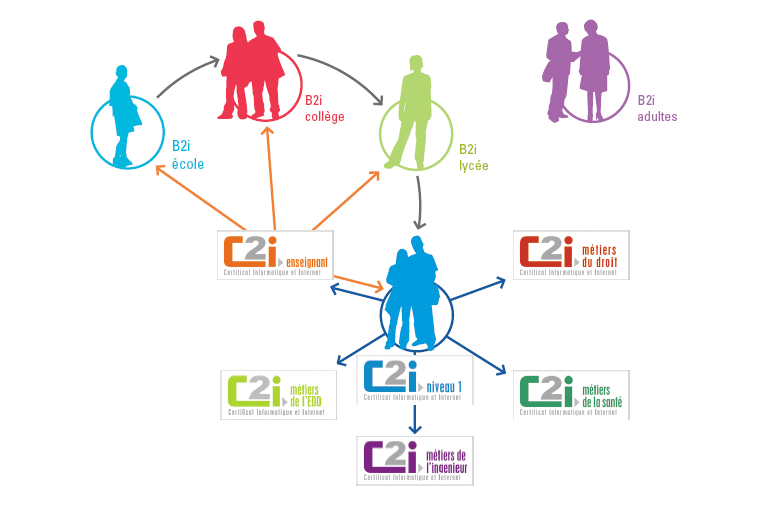
\includegraphics[width=\linewidth]{../resources/illustrations/c2i}};
		\node[draw=none,below of = image, node distance=3.5cm] {
			{\tiny \it \color{black!30} \url{http://sti.ac-montpellier.fr/spip.php?rubrique1068}}
		};
	\end{tikzpicture}
	  \footlineextra{\cite{b2i_c2i}}
\end{frame}

\begin{frame}{Opérations portables}
	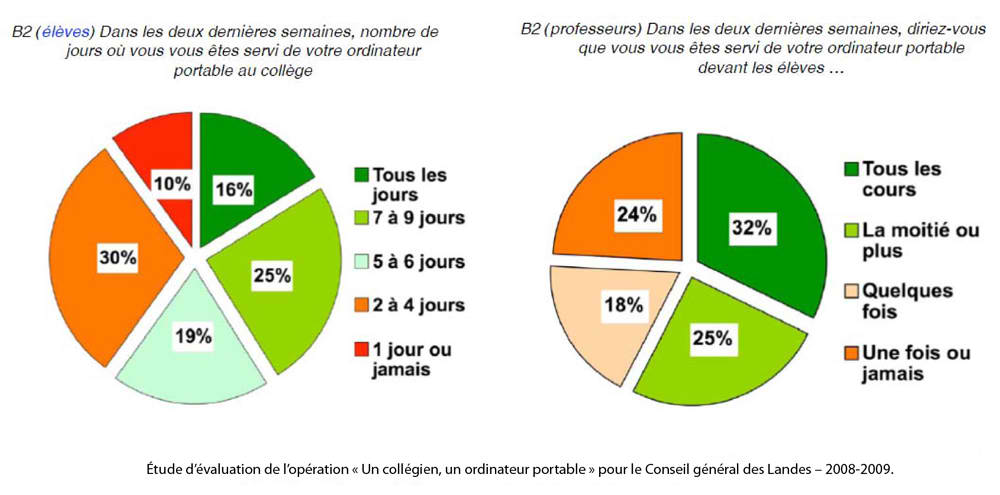
\includegraphics[width=\linewidth]{../resources/illustrations/usage_portables}
	  \footlineextra{\cite{portables35}\cite{portables40}\cite{portables60}}
\end{frame}

\begin{frame}{Organisations et colloques internationaux}
	\begin{tikzpicture}
	  	\node (image) {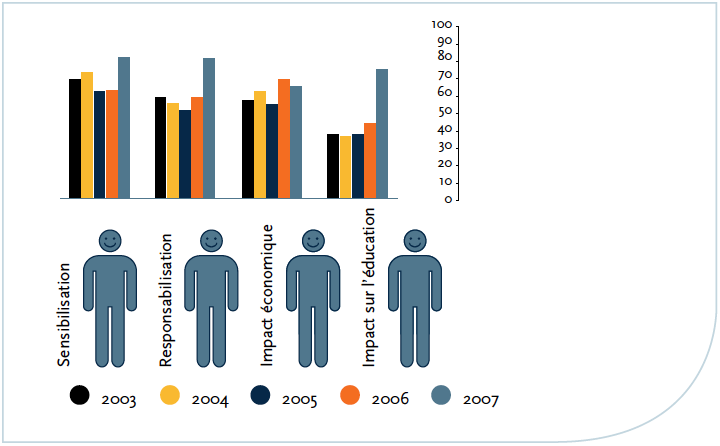
\includegraphics[width=\linewidth]{../resources/illustrations/impact_iicd}};
		\node[draw=none,below of = image, node distance=3.5cm] {
			{\tiny \it \color{black!30} Impact des projets en éducation soutenus par l'IICD sur les utilisateurs finaux 2003-2007.}
		};
	\end{tikzpicture}
	\footlineextra{\cite{educ_forum}\cite{tics}\cite{peixoto2006regard}}
\end{frame}

\begin{frame}{Refondons l'école de la république}

\begin{block}{Rapport piloté par}
  \begin{itemize}
  \item François Bonneau
  \item Marie-Françoise Colombani
  \item Christian Forestior
  \item Nathalie Mons
  \end{itemize}
\end{block}

\footlineextra{\cite{rapport_ecole_2012}}
\end{frame}


\begin{frame}{Refondons l'école de la république}

\begin{block}{Idées}
  \begin{itemize}
    \item l’objectif est désormais d’apprendre à apprendre
    \item les langues doivent faire l’objet d’une appropriation active
    \item renforcés les usages pédagogiques du numérique en primaire
   \item Pratiquer, plutôt qu’une notation sanction, une évaluation positive simple et lisible
  \end{itemize}
\end{block}
\footlineextra{\cite{rapport_ecole_2012}}
\end{frame}

\begin{frame}{Refondons l'école de la république}
\begin{block}{Actions}
\begin{itemize}
  \item Inscrire dans la loi l’éducation aux médias et à l’information 
  \item Former les personnels aux usages pédagogiques du numérique
  \item Mettre en place une politique de recherche dans le cadre des applications
pédagogiques du numérique
\end{itemize} 
\footlineextra{\cite{rapport_ecole_2012}}
\end{block}


\end{frame}

\subsection{Autres acteurs}

\begin{frame}{Moodle}
\end{frame}

\begin{frame}{E-Learning}

\begin{itemize}
\item Khan Academy
\item Udacity (ai-class.com)
\item Coursera (ml-class.org)
\item \url{http://www.youtube.com/education}
\end{itemize}

\end{frame}

\begin{frame}
  \personality{Nicholas Negroponte}{../resources/illustrations/nicholasnegroponte}{%
    \begin{itemize}
      \item Professeur au MIT
      \item Fondateur du MediaLab (1985)
      \item Lancement de Wired
    \end{itemize}
  }
   \pause
   \begin{block}{Centres d'intérêts}
     \begin{itemize}
       \item Art + Math $\rightarrow$ Architecture MIT
       \item Art + Sciences $\rightarrow$ Ordinateurs
     \end{itemize}
     $\Rightarrow$ MIT MediaLab (1985)
   \end{block}
       \footlineextra{\cite{wikipedia_nicholas_negroponte}\cite{ted_olpc_2006}\cite{ted_olpc_2008}}
\end{frame}

\begin{frame}{One Laptop Per Child}
      % Puis il quitte le poste de président du MediaLab dans les année 2000 avec la volonté de mener un projet important
  \begin{block}{OLPC (2005)}
        S'occuper de l'éducation en agissant sur les enfants.
        \onslide<2->{
    \begin{itemize}
      \item But non lucratif
      \item Conception \& fabrication d'un ordinateur
      \item Distribution aux enfants
      \item Connexion haut débit
    \end{itemize}
    }
    \onslide<3->{
    Projet basé sur la philosophie du \og constructionnisme \fg{}, avec Seymour Papert.}
  \end{block}
  \begin{center}
  \onslide<2->{
    
\includegraphics[width=.6\textwidth]{../resources/illustrations/OLPC_logo}
    }
  \end{center}
       \footlineextra{\cite{ted_olpc_2006}\cite{ted_olpc_2008}}
\end{frame}

\begin{frame}{One Laptop Per Child}
\includegraphicsabsolute{../resources/illustrations/olpc_mesh}{3.5cm}{.2cm}{1.6cm}
\includegraphicsabsolute{../resources/illustrations/olpc2}{8cm}{5cm}{0.7cm}
\includegraphicsabsolute{../resources/illustrations/olpc1}{3cm}{0cm}{6.5cm}
\includegraphicsabsolute{../resources/illustrations/olpc_display}{3.2cm}{2.3cm}{4.3cm}

       \footlineextra{\cite{ted_olpc_2006}\cite{ted_olpc_2008}}
\end{frame}

\begin{frame}{One Laptop Per Child}
  \begin{itemize}
   \item Nicholas  Negroponte, fondateur du MediaLab (MIT)
   \item Inspiration du Dynabook d'Alan Kay
   \item 1986 (présenté en 1978) : Seymour Papert à fait l'observation suivante [Teaching childs thinking \footnote{\texttt{http://stager.org/articles/teachingchildrenteaching.pdf}}] : les enfants qui écrivent des programmes informatique comprennent les choses différemment, et quand ils les debug, ils arrivent presque à apprendre sur l'apprentissage.
   \item FINALITÉ : faire programmer les enfants ! -> Squeak LOGO 
   \item 1982 : travail avec Seymour Papert : les premier à apporter des ordinateurs aux écoles des pays en voie de développement
  \end{itemize}
  Souhait de Nicholas de fonder un projet important lors de son départ du Medialab : OLPC. L'idée est de s'occuper d'éducation en agissant sur les enfants :
  \begin{itemize}
  \item en leur apportant l'accès aux ordinateurs,
  \item 
  \end{itemize}
  -> Les enfant y arrivent aussi bien qu'ici
    \footlineextra{\cite{ted_olpc_2006}\cite{ted_olpc_2008}}
\end{frame}

\begin{frame}
    \personality{Sugata Mitra}{../resources/illustrations/sugatamitra}{%
        \begin{itemize}
          \item Professeur à l'université de Newcastle,
          \item Domaines
          \begin{itemize}
            \item Techniques d'éducation,
            \item Sciences du langage et de la communication,
            \item Physique (PhD).
          \end{itemize}
        \end{itemize}
        }
    \pause
    \begin{block}{Hole in the wall}
    \begin{coolquote}[Sugata Mitra, Conférence TED \textit{The child-driven education}]
    Les bons enseignants ne veulent pas aller dans les endroits où on a le plus besoin d'eux
    \end{coolquote}
    
      Fournir un libre accès aux ordinateurs et à Internet.
      \center 1999 $\rightarrow$ New Delhi
    \end{block}
  \footlineextra{\cite{wikipedia_sugata_mitra}\cite{website_hole_in_the_wall}\cite{ted_mitra_1,ted_mitra_2}}
\end{frame}

\begin{frame}{Hole In the Wall (HIW)}
\begin{center}
  \begin{minipage}{0.45\textwidth}
    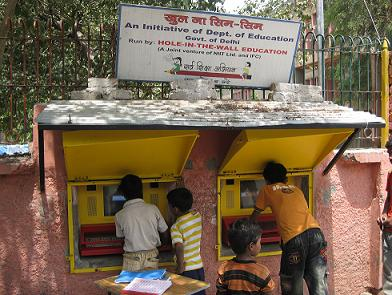
\includegraphics[width=\textwidth]{../resources/illustrations/hiw_1.jpg}\\
    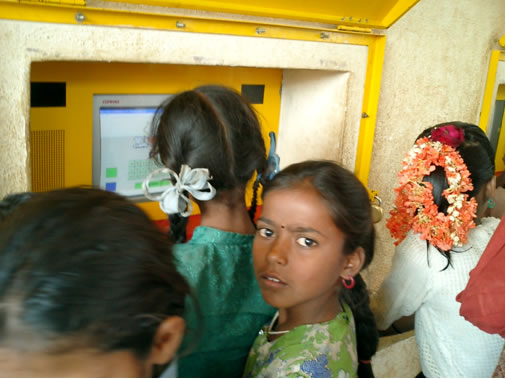
\includegraphics[width=\textwidth]{../resources/illustrations/hiw_2.jpg}
  \end{minipage}
  \begin{minipage}{0.45\textwidth}
    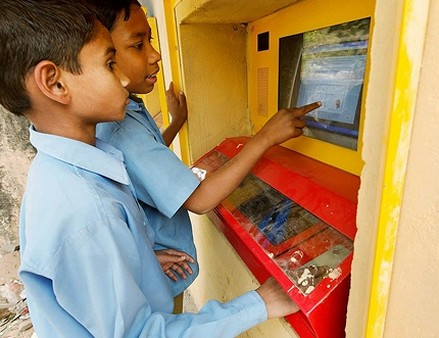
\includegraphics[width=\textwidth]{../resources/illustrations/hiw_3.jpg}\\
    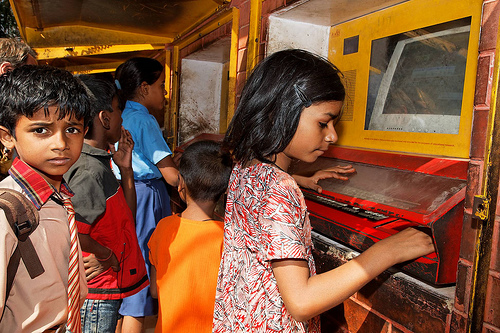
\includegraphics[width=\textwidth]{../resources/illustrations/hiw_4.jpg}
  \end{minipage}
\end{center}
  \footlineextra{\cite{ted_mitra_1}\cite{ted_mitra_2}}
\end{frame}

\begin{frame}{Hole In the Wall (HIW)}
  \begin{block}{Observations}
    \begin{itemize}
      \item Échange entre les enfants
      \item Volonté d'apprendre
    \end{itemize}
    $\Rightarrow$ Des groupes d'enfants peuvent apprendre à utiliser les ordinateurs et Internet seuls.
  \end{block}
    \footlineextra{\cite{ted_mitra_1}\cite{ted_mitra_2}}
\end{frame}

\begin{frame}{Hole In the Wall (HIW)}
  \begin{block}{Étape 2}
    \begin{itemize}
      \item Apprentissage de l'Anglais
      \item Fort accent Télougou
      \item Logiciel de reconnaissance vocale
    \end{itemize}
  \end{block}
\pause
  \begin{block}{Deux mois plus tard\ldots}
    Accent très proche de l'anglais Britannique.
    
    $\Rightarrow$ Si l'enfant est intéressé, l'éducation se produit.
  \end{block}
    \footlineextra{\cite{ted_mitra_1}\cite{ted_mitra_2}}
\end{frame}

\begin{frame}{Hole In the Wall (HIW)}
\begin{block}{Observation deux ans après\ldots}
  Utilisation intensive des ressources Internet pour réaliser les devoirs.
\end{block}
\pause
\begin{coolquote}[Sugata Mitra, Conférence TED \textit{The child-driven education}]
Si il y a plein de trucs sur Google, pourquoi aurions-nous besoin de se les bourrer dans notre tête ?
\end{coolquote}
\pause
  \begin{block}{Étape 3}
    \begin{itemize}
      \item Apprentissage de la biotechnologie
      \item 26 enfants de 12 ans
      \item Ne parlent que Tamoul
      \item Ordinateurs + ressources en anglais
    \end{itemize}
  \end{block}
    \footlineextra{\cite{ted_mitra_1}\cite{ted_mitra_2}}
\end{frame}

\begin{frame}{Hole In the Wall (HIW)}
  \begin{block}{Deux mois plus tard\ldots}
    Les enfants disaient n'avoir rien appris.
    \pause
    
    \begin{coolquote}[Écolière Indienne]
    À part le fait qu'une mauvaise réplication de la molécule d'ADN provoque des maladies génétiques, nous n'avons rien compris
    \end{coolquote}
    Observations
    \begin{itemize}
      \item Prise du rôle d'enseignant
      \item Score $\nearrow$ 30\%
    \end{itemize}
  \end{block}
    \footlineextra{\cite{ted_mitra_1}\cite{ted_mitra_2}}
\end{frame}

\begin{frame}{Hole In the Wall (HIW)}
  \begin{block}{Étape 4}
    Méthode grand-mère :
    \begin{itemize}
      \item S'assoir
      \item Les admirer
      \item Les encourager
    \end{itemize}
  \end{block}
  \pause
  \begin{block}{Deux mois plus tard\ldots}
  \begin{tabular}{l c l}
  30\% $\nearrow$ 50\% &=& Moyenne avec le système éducatif traditionnel \\
  \end{tabular}
  \end{block}
    \footlineextra{\cite{ted_mitra_1}\cite{ted_mitra_2}}
\end{frame}

\begin{frame}{Hole In the Wall (HIW)}
  \begin{block}{Étape 5 (2009)}
  32 élèves de Gateshead (Inde).
    Mise en place d'une méthode :
    \begin{itemize}
      \item Groupes de 4
      \item Un seul ordinateur par groupe
      \item Possibilité de changer de groupes
      \item Possibilité de copier les autres groupes
      \item Accès à Internet
    \end{itemize}
    $\rightarrow$ 6 question du GCSE
  \end{block}
  \pause
  \begin{block}{Résultats}
  \begin{tabular}{l c l}
    \begin{minipage}{0.5\textwidth}
      \begin{itemize}
        \item Meilleur groupe : 22mn
        \item Dernier groupe : 45mn
      \end{itemize}
    \end{minipage} &  $\rightarrow$ & 76\% de réussite \\
    \end{tabular}
  \end{block}
    \footlineextra{\cite{ted_mitra_1}\cite{ted_mitra_2}}
\end{frame}

\begin{frame}{Hole In the Wall (HIW)}

  S'agit-il d'apprentissage ?
  \pause
  \begin{block}{Deux mois plus tard\ldots}
    Réalisation d'un contrôle traditionnel\pause $\rightarrow$ 76\% de réussite.
    
    $\Rightarrow$ Mémoire photographique
  \end{block}
    \footlineextra{\cite{ted_mitra_1}\cite{ted_mitra_2}}
\end{frame}

\begin{frame}{Hole In the Wall (HIW)}
  Généralisation de ses travaux.
  \pause
  \begin{block}{Granny Cloud}
    Grands-mères Britanniques $\leftrightarrow$ Skype $\leftrightarrow$ Enfants Indiens
    \begin{itemize}
      \item 200 Grands-mères
      \item 1 heure par semaine
    \end{itemize}
  \end{block}
  \pause
    \begin{block}{SOLEs}
    Self Organised Learning Environments
  \end{block}
    \footlineextra{\cite{ted_mitra_1}\cite{ted_mitra_2}}
\end{frame}

\begin{frame}{Hole In the Wall (HIW)}
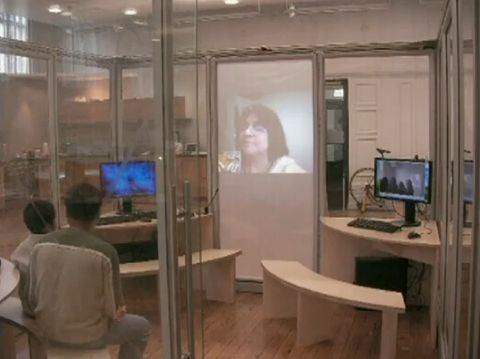
\includegraphics[width=.9\textwidth]{../resources/illustrations/soles.jpg}
  \footlineextra{\cite{ted_mitra_1}\cite{ted_mitra_2}}
\end{frame}

\begin{frame}{Hole In the Wall (HIW)}
  \begin{block}{Conclusion}
    Apparition de systèmes auto-organisés
    \begin{itemize}
      \item Apparition d'une structure
      \item Émergence
    \end{itemize}
    \pause
    \begin{center}
      $\Downarrow$
      
     \begin{coolquote}[Sugata Mitra, Conférence TED \textit{The child-driven education}]
      L'éducation est un système auto-organisé, dans lequel l'apprentissage est un phénomène émergent
    \end{coolquote}
    \end{center}
  \end{block}
    \footlineextra{\cite{ted_mitra_1}\cite{ted_mitra_2}}
\end{frame}

\subsection{Quelles solutions ?}

\begin{frame}{À plusieurs niveaux}
\begin{block}{Enseignements}
Nécessité de former les jeunes aux nouvelles technologies, aux aspects techniques mais aussi et surtout les éduquer face aux dangers que représente la société hyper-connectée d'aujourd'hui.
\end{block}
\begin{block}{Méthodes}
Revoir les méthodes d'apprentissages afin de profiter pleinement des TIC dans nos écoles, cela exige une remise en question majeure du système et des méthodes éducatives actuels.
\end{block}
\end{frame}


\begin{frame}{Enseignements}
  \begin{block}{l'image}
    \begin{itemize}
      \item omniprésence de l'image dans les médias
      \item nécessité d'une formation à la lecture de l'image
    \end{itemize}
  \end{block}
\footlineextra{\cite{book_serusclat}}
\end{frame}
  
\begin{frame}{Enseignements}
  \begin{block}{Éducation sur les risques des NTIC}
    \begin{itemize}
      \item publicisation de la vie privé
      \item marchandisation des données personnelles
      \item (faite de façon constructivisme)
    \end{itemize}
  \end{block}
\end{frame} 



\begin{frame}{Enseignements}
\Huge \textbf{:)}
\end{frame}

\begin{frame}{Méthodes}
\textbf{\Huge  S'appuyer sur le constructi[visme|onisme] ?}
\begin{itemize}
  \item \textbf{Constructivisme 1923 - Piaget}. On suppose que les individus ne perçoivent pas une copie de la réalité qui les entours, mais une reconstruction interne. L'individu reconstruit en permanance les objets perçus en fonction des concept déjà intégrés.
  \item \textbf{Constructionnisme 1960 - Seymour Papert}. En accord avec le constructivisme mais met en évidence l'importance de la construction d'une "entité publique" comme le dialogue et l'interaction. Rôle des constructions réelles dans les constructions mentales.
\end{itemize}
\end{frame}

\begin{frame}
  \personality{Jean Piaget}{../resources/illustrations/piaget}{%
    \begin{itemize}
      \item Psychologie du développement
      \item Développement du constructivisme (1923)
      \item Stades (évolution individuelle)
    \end{itemize}
  }
  \begin{center}  
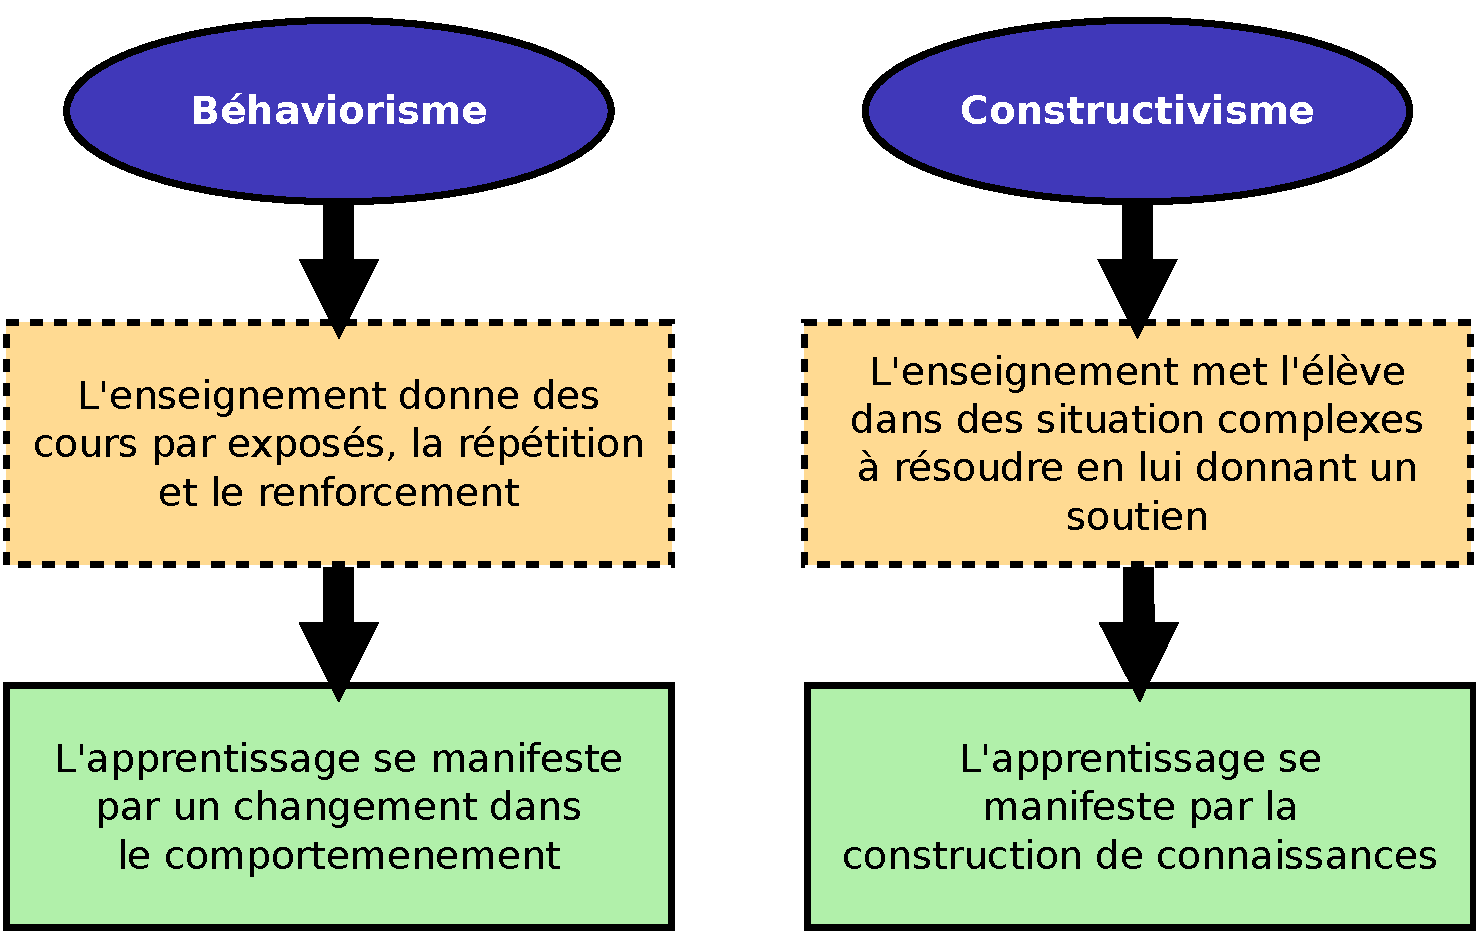
\includegraphics[width=.8\textwidth]
  {../resources/illustrations/behaviorisme_constructivisme}
    \end{center}
  \footlineextra{\cite{wikipedia_piaget,wikipedia_constructivisme}}
\end{frame}

\begin{frame}
  \personality{Seymour Papert}{../resources/illustrations/papert}{%
    \begin{itemize}
      \item Informaticien \& Mathématicien
      \item Deux doctorats (Mathématique)
      \item Chercheur au MIT (1963)
      \item Création de l'équipe \og Groupe de Recherche sur l'Épistémologie et l'Apprentissage \fg{} (MIT MediaLab)
    \end{itemize}
  }  
  \footlineextra{\cite{wikipedia_papert}}
\end{frame}

\begin{frame}{Constructionnisme}
  \emph{\centering\huge Constructionnisme $\neq$ Instructionnisme}
  \footlineextra{\cite{book_seymour_papert}}
\end{frame}

\begin{frame}{Constructionnisme}

\begin{columns}[T]
\begin{column}[l]{.5\textwidth}
  \begin{block}{Théorie de l'apprentissage}
  Notions
    \begin{itemize}
      \only<1,3->{\item de \og Hard fun \fg{}}
      \only<2>{\item \textbf{de \og Hard fun \fg{}}}
      \only<1-2,4->{\item d'interactions et de\\groupe}
      \only<3>{\item \textbf{d'interactions et de\\groupe}}
      \only<1-3,5->{\item de \og bricolage \fg{} et du \og bricoleur \fg{}}
      \only<4>{\item \textbf{de \og bricolage \fg{} et du \og bricoleur \fg{}}}
      \only<1-4>{\item d'\og apprendre à\\apprendre \fg{}}
      \only<5>{\item \textbf{d'\og apprendre à\\apprendre \fg{}}}
    \end{itemize}
  \end{block}
\end{column}
\begin{column}[l]{.5\textwidth}
  \only<2>{
    \begin{block}{\og Hard Fun \fg{}}
      \begin{itemize}
        \item Se lancer des Challenges
        \item Sport $\rightarrow$ fun \& difficile
      \end{itemize}
      $\nRightarrow$ Fun malgré la difficulté\\
      \textbf{$\Rightarrow$ Fun grâce à la difficulté}
    \end{block}
  }
  \only<3>{
    \begin{block}{Interaction \& groupe}
      \begin{itemize}
        \item Dialogues et échanges $\rightarrow$ groupe
        \item Construction dans le réel $\rightarrow$ favorisé par la programmation
      \end{itemize}
    \end{block}
  }
  \only<4>{
    \begin{block}{\og Bricolage \fg{}}
    \textit{La pensée sauvage}, Claude Lévi-Strauss (1962)
      \begin{itemize}
        \item Science du concret vs. Science analytique (abstrait)
        \item Tel un bricoleur qui répare quelque chose avec \og ce qu'il a sous la main \fg{}
      \end{itemize}
      $\Rightarrow$ favorisé par la programmation
    \end{block}
  }
  \only<5>{
    \begin{block}{Apprendre à apprendre}
      Résultat des points précédents.
    \end{block}
    \vfill
      \begin{coolquote}[Seymour Papert \cite{book_seymour_papert}]
    Le savoir dont les enfants ont le plus besoin est celui qui leur permet d'en acquérir davantage
  \end{coolquote}
  }
\end{column}
\end{columns}
    \footlineextra{\cite{interview_papert,book_seymour_papert}}
\end{frame}

\begin{frame}{LOGO (1967)}
  \og Lisp sans parenthèses \fg{}
  
  \includegraphicsabsolute{../resources/illustrations/logo_logo}{4cm}{7cm}{2cm}

  \begin{description}
    \item $\rightarrow$ NetLogo
    \item $\rightarrow$ Smalltalk
    \item $\rightarrow$ Scratch
  \end{description}
  \begin{block}{Applications}
    \begin{itemize}
      \item Dessin à l'écran
      \item Contrôle de la tortue
      \item Musique
    \end{itemize}
  \end{block}
  \footlineextra{\cite{wikipedia_papert}}
\end{frame}

\begin{frame}{LOGO}
  \includegraphicsabsolute{../resources/illustrations/logo_screen}{6cm}{.2cm}{1.6cm}
  \includegraphicsabsolute{../resources/illustrations/logo_turtle_1}{6.5cm}{6.6cm}{.68cm}
  \includegraphicsabsolute{../resources/illustrations/logo_turtle_3}{6.2cm}{.2cm}{5cm}
\end{frame}

\begin{frame}
  \begin{center}
    \vspace{.4cm}
    \emph{\huge L'informatique}
    \vspace{-.4cm}
  \end{center}
  \begin{columns}[T]
    \begin{column}[l]{.5\textwidth}
      \begin{block}{\og Information Technology \fg{}}
        Accès à l'information.
        
        $\Rightarrow$ Aspect \emph{informationnel}
      \end{block}
    \end{column}
    \begin{column}[l]{.5\textwidth}
      \begin{block}{\og Computer Science\fg{}}
        Manipulation de données
        
        $\Rightarrow$ Aspect \emph{constructionnel}
      \end{block}
    \end{column}
  \end{columns}
  \pause  
  \begin{center}
    \vspace{.4cm}
    \emph{\huge L'éducation}
    \vspace{-.4cm}
  \end{center}
  \begin{columns}[T]
    \begin{column}[l]{.5\textwidth}
      \begin{block}{Acquisition d'informations}
        Délivrer de l'information. Ex :
        \begin{itemize}
          \item Histoire
          \item Géographie
          \item \ldots
        \end{itemize}
        $\Rightarrow$ Aspect \emph{informationnel}
      \end{block}
    \end{column}
    \begin{column}[l]{.5\textwidth}
      \begin{block}{Art / Technique / Créatif}
        Construction d'une entité. Ex :
        \begin{itemize}
          \item Raisonnement / Concepts
          \item Musique / Dessin
          \item \ldots
        \end{itemize}
      $\Rightarrow$ Aspect \emph{constructionnel}
      \end{block}
    \end{column}
  \end{columns}
  
  \footlineextra{\cite{interview_papert}}  
\end{frame}

\begin{frame}{Méthodes d'apprentissage}
\begin{itemize}
  \item Une personne motivée réussira à apprendre par elle même
  \item Nécessité de constructions réelles pour l'assimilation (la construction / amélioration) des nouveaux concepts mentaux
  \item Idée de bricoler les concept. Terme introduit Claude Lévi-Strauss dans \textit{La pensée sauvage}. % Le bricolage s'oppose à la pensée unique (méthode analytique) instruite dans le système éducatif traditionnel. Idée de bricolage (terme repris de Lévi-Strauss, Pensées sauvages) est de travailler sur du concret afin d'arriver à un résultat de manière détournée (comme le ferait un bon bricoleur).
  \item L'ordinateur donne de nombreuses opportunités de bricolages.
  \item Le constructionnisme s'oppose à l'insctructionnisme.
  \begin{description}
    \item[Instructionnisme : ]affirme la croyance que pour améliorer l'apprentissage il faut développer l'instruction (enseigner mieux).
    \item[Constructionnisme : ]favoriser le plus grand apprentissage avec le moins d'enseignement possible.
    \end{description}
    \og{}Le savoir dont les enfants ont le plus besoin est celui qui leur permet d'en acquérir davantage\fg (Papert p.141).
\end{itemize}
\end{frame}

\begin{frame}{Concrètement}
\begin{itemize}
  \item D'abord confronter l'élève à la problématique avant de lui enseigner les concepts abstraits
  \item Réaliser des projets plutôt que résoudre des problèmes
  \item 
\end{itemize}
\end{frame}

\begin{frame}{Méthodes d'apprentissage}
  \begin{block}{Prise en compte des avancées en neurosciences}
    \begin{itemize}
    \item faire un résumé en fin de cours
    \item création de carte mentale \\[10pt]
    \end{itemize}
  \end{block}
    
  \begin{center}
    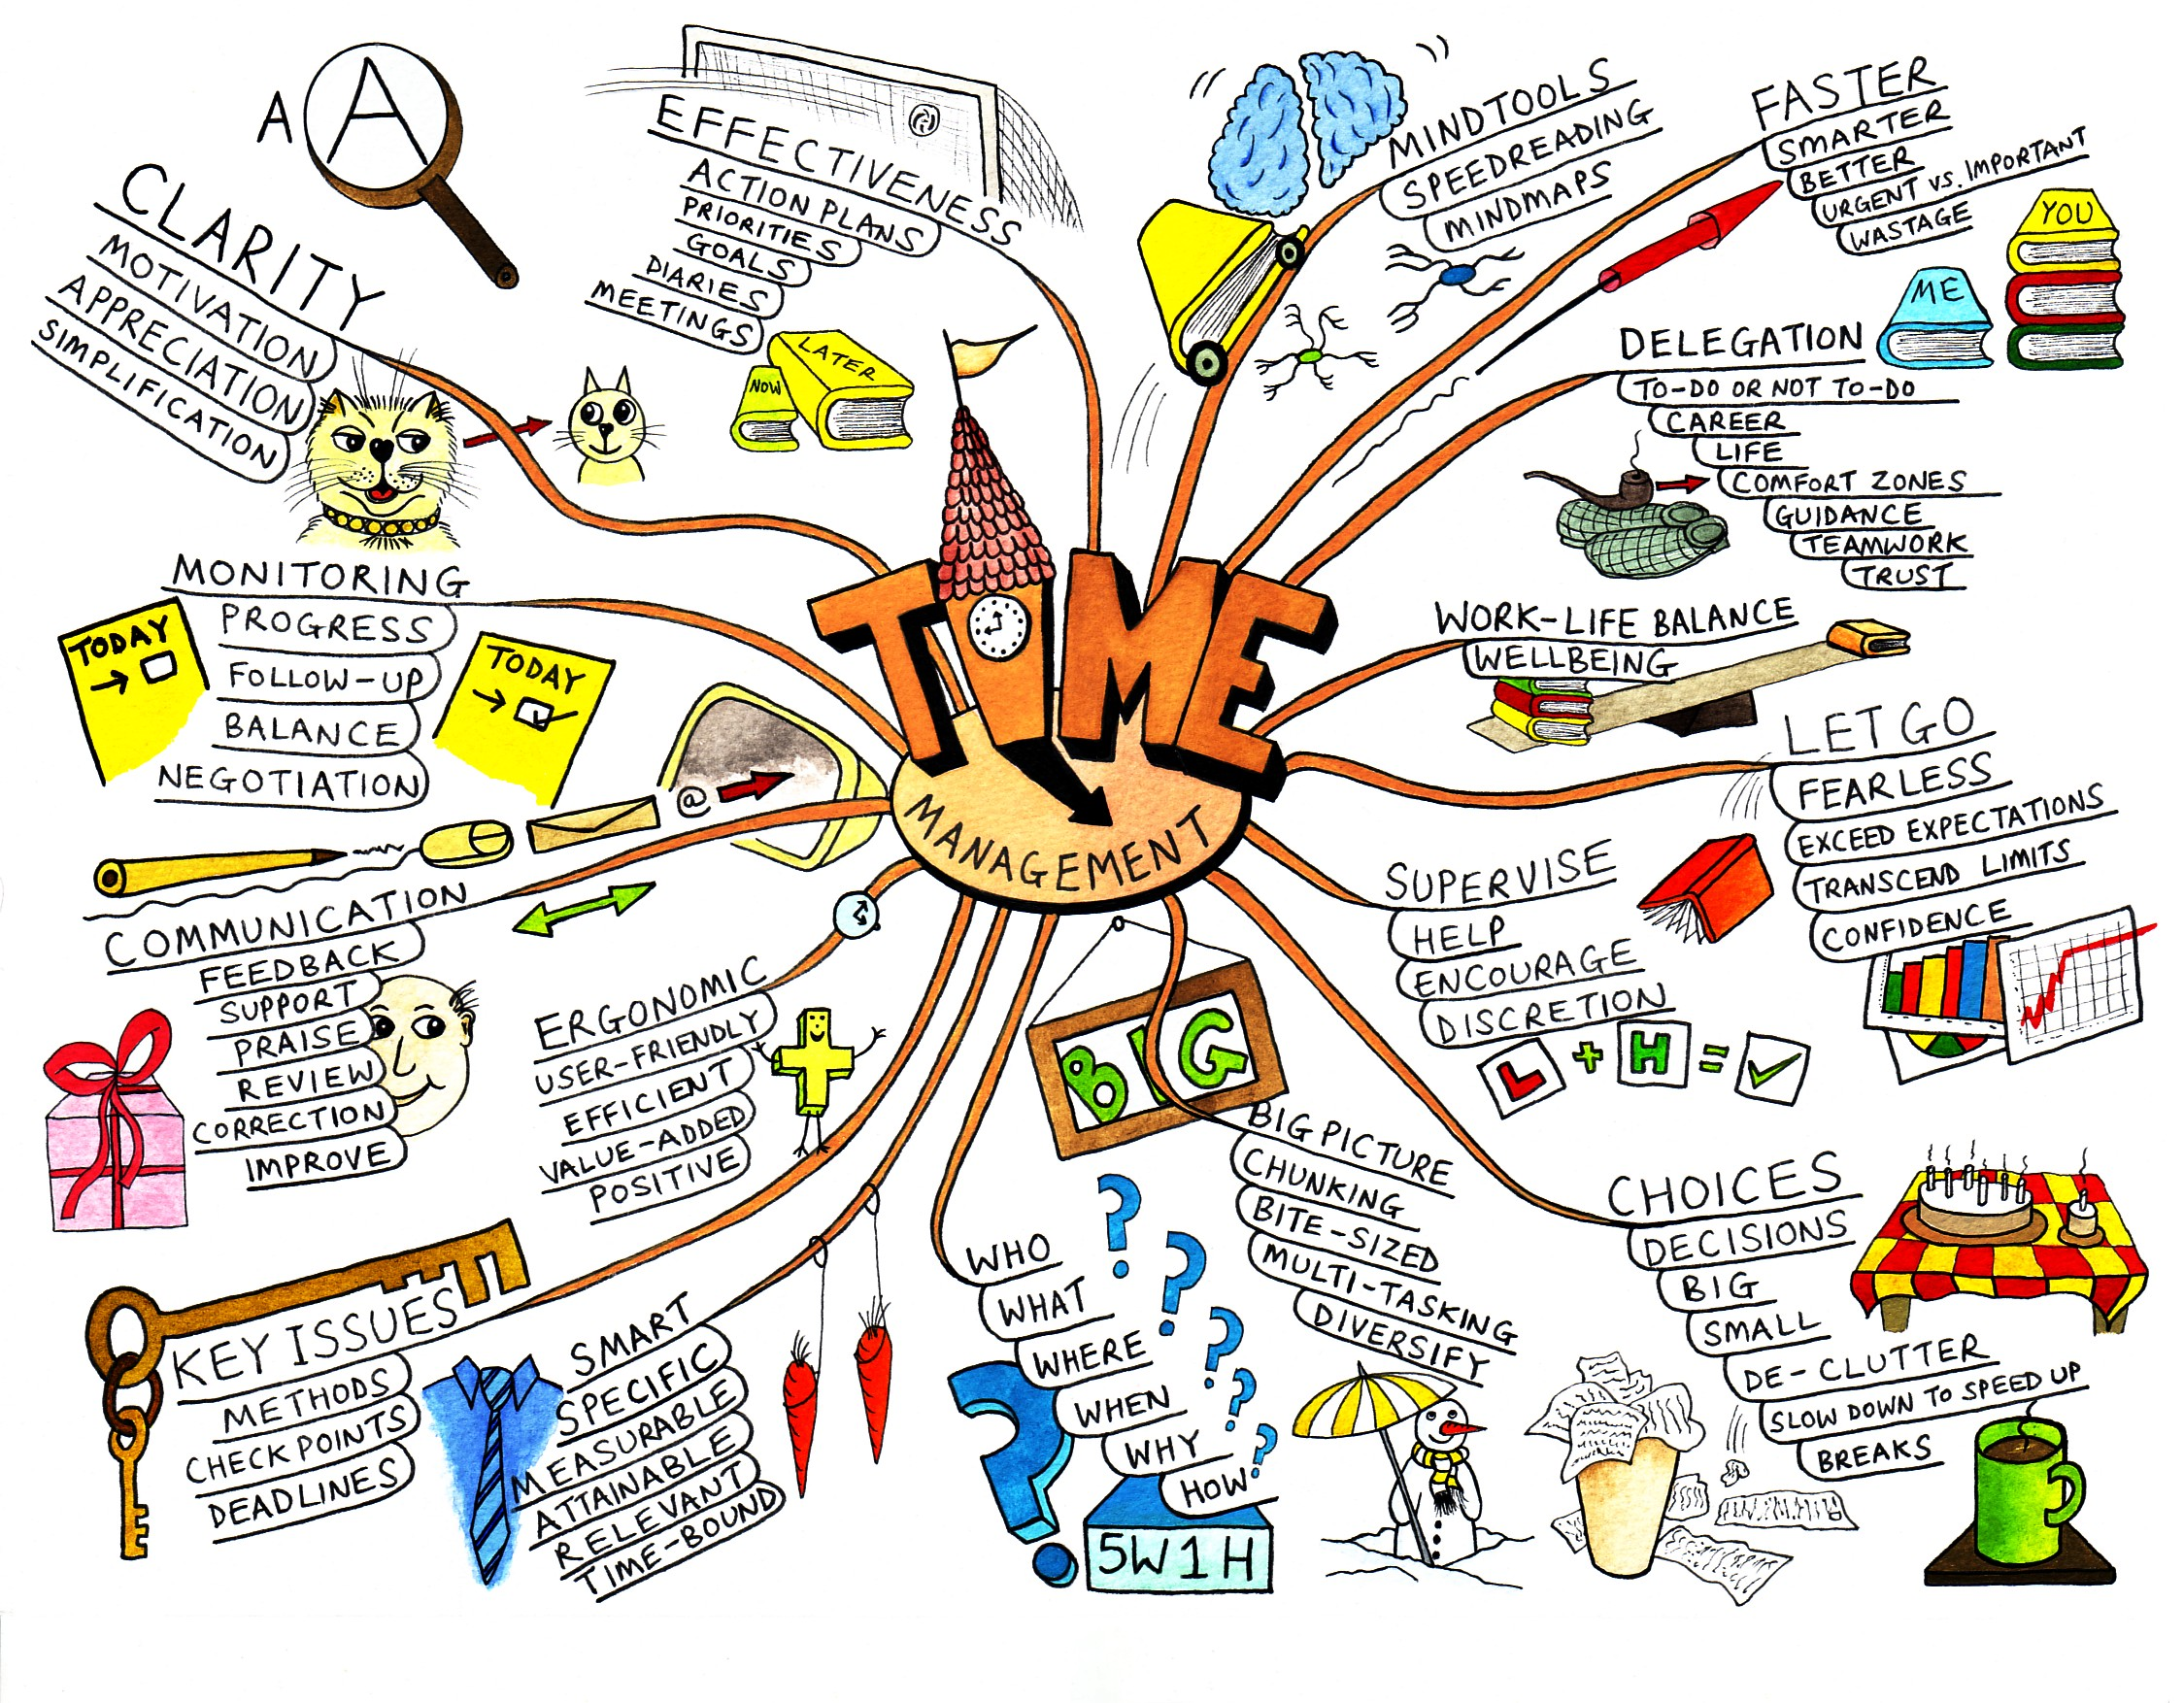
\includegraphics[width=.6\textwidth]{../resources/illustrations/mindmap.jpg}
  \end{center}

  \footlineextra{\cite{neurosup}}
\end{frame}
